\section{Distribution of the Fluctuations}\label{sec:5.3}

The energy deviation $\epsilon$ at any instant $t$ is the result of a superposition of the
contributions from the emission of quanta at all earlier times $t_i$. We may in fact, write for $\epsilon(t)$
\begin{align} \label{eq:5.49}
	\epsilon(t) = \sum_{t_i<t} u_i e^{-(t-t_i)\tau_\epsilon}\cos\Omega(t-t_i),
\end{align}
where $u_i$ is the energy of the quantum emitted at $t_i$. Since the typical value of $\epsilon(t)$ is much larger than the typical quantum energy -- see Eq.~\eqref{eq:5.32} -- and since the times $t_i$ are randomly distributed, the sum at any instant $t$ consists of contributions from a large number of small terms which are all statistically independent, and which are positive and negative with equal probability. It is well known\footnote{And follows from the Central Limit Theorem of probability theory.} that the result of such a sum is a stochastic quantity whose most probable value is zero and which is otherwise distributed as a normal error function -- a so-called Gaussian distribution. That is the probability $w(\epsilon)d\epsilon$ that the energy deviation
will be found in an interval $d\epsilon$ at $\epsilon$ is distributed according to
\begin{align}\label{eq:5.50}
	w(\epsilon)d\epsilon = \dfrac{1}{\sqrt{2\pi}\sigma_\epsilon} \exp{(-\epsilon^2/\sigma_\epsilon^2)}d\epsilon.
\end{align}
The parameter $\sigma_\epsilon$, often called the standard deviation, is equal to the root-mean-
Square spread of the distribution -- that is, the square root of $\mean{\epsilon^2}$ -- as can
easily be shown by a direct integration:
\begin{align}
	\sigma_\epsilon^2 = \int_{-\infty}^{\infty} \epsilon^2 w(\epsilon) d\epsilon.
\end{align}
(The distribution function $w(\epsilon)$ is properly normalized so that its complete integral
is equal to 1) The standard deviation $\sigma_\epsilon$ is then, the same quantity we have evaluated in the preceding section.\\
In a stored beam we have, normally, a large number $N$ of stored electrons. So long as any interactions among them can be ignored, the distribution of energies within the bunch will -- under stationary conditions -- also be described by Eq.~\eqref{eq:5.40}. That is, the number of electrons with energies between $\epsilon$ and $\epsilon+d\epsilon$ will be just $Nw(\epsilon)d\epsilon$. And the ``half-width'' of the spread of energies in the beam is described by $\sigma_\epsilon$.\\
The distribution function of Eq.~\eqref{eq:5.50} and also our calculation of $\sigma_\epsilon$ assume that the energy oscillations are linear (with nonlinearities, Eq.~\eqref{eq:5.49} is not
correct and the effects of the individual quanta are no longer independent). We have already seen however, that the energy oscillations are not linear for large energy deviations. If the rf voltage function is significantly nonlinear over the time displacements that correspond to the likely energy deviations, we must expect the probability distribution for $\epsilon$ to be distorted from the ideal distribution of Eq.~\eqref{eq:5.50}. If, however, the nonlinearity
 is not too great over the largest part of the distribution, we may expect that neither $\sigma_\epsilon$; nor the distribution function of the energy deviations will be affected very much.\\
The distribution of energy deviations just considered implies related distributions in other parameters of the energy oscillations. The relationships are most easily understood by considering the electron's trajectory in a ``phase diagram'' such as the one discussed in Section~\ref{sec:3.5}. Suppose we describe the state of the energy oscillation by giving its energy deviation $\epsilon$ and its ``scaled'' time displacement $\theta$, which we define by
\begin{align} \label{eq:5.52}
	\theta = \dfrac{\Omega E_0}{\alpha} \tau.
\end{align}
$\Omega$, the angular frequency of the energy oscillation and $\alpha$, the dilation factor are
constants so $\theta$ is just a scaled equivalent of $\tau$ the time displacement coordinate of
the energy oscillations (See Section~\ref{sec:3.5}). So long as the damping rate is small, $\theta$ could equally well be defined by
\begin{align}
	\theta = \dfrac{1}{\Omega} \dfrac{d\epsilon}{dt},
\end{align}
so it may also be viewed as a normalized derivative of $\epsilon$. We may now represent the state of motion of an electron by a point on a two-dimensional graph in which $\epsilon$ and $\theta$ are orthogonal coordinates -- see Fig.~\ref{fig:fig44}(a) -- and in which an oscillation
of constant amplitude would describe a circle. Then so long as the damping and the quantum effects are small, we may consider that for any small interval of time, $\epsilon$ and $\theta$ vary as
\begin{align}
	\epsilon &= A \cos\varphi,\\
    \theta &= A \sin\varphi;
\end{align}
where
\begin{align}
	\varphi = \Omega t - \varphi_0,
\end{align}
and $A$ is slowly varying amplitude. The quantities $A$ and $\varphi$ are a polar representation of the representative point and $\varphi$ increases as $\Omega t$.
\begin{figure}[!htb]
	\centering
	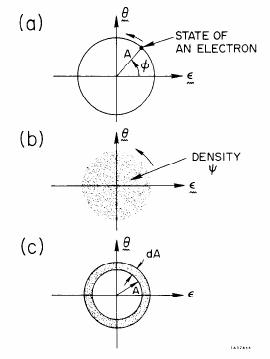
\includegraphics[width=0.8\linewidth]{./Figuras/fig44.jpeg}
	\caption{Scaled phase space of the energy oscillations.}
	\label{fig:fig44}
\end{figure}
The distribution of energy oscillations of the electrons in a stored bunch can now be represented
 by a distribution of points in the phase plot as indicated schematically in Fig.~\ref{fig:fig44}b. A complete description of the distribution is given by specifying the density $\Psi(\epsilon,\theta)$ in the $\epsilon,\theta$ plane. That is $\Psi(\epsilon,\theta) d\epsilon d\theta$ is to represent the number of electrons found in the element of area $d\epsilon d\theta$ located at $(\epsilon,\theta)$. We already know the projection of $\Psi(\epsilon,\theta)$ on the horizontal axis. If there are $N$ electrons in the bunch it is just $N w(\epsilon)$. But in one-quarter of an oscillation each electron rotates one-quarter of a revolution about the origin of the figure. And since we are assuming a stationary distribution
 -- that is one with no time variations -- the projection on the vertical and on the horizontal
 axes must be identical. It must be then, that the number of electrons in an element of area $d\epsilon d\theta$ is given by
\begin{align} \label{eq:5.57}
	\Psi(\epsilon,\theta)d\epsilon d\theta = \dfrac{N}{2\pi \sigma_\epsilon^2} \exp\left( -\dfrac{\epsilon^2 + \theta^2}{2\sigma_\epsilon^2} \right) d\epsilon d\theta.
\end{align}
The projection on the horizontal axis is
\begin{align}
	\int_{-\infty}^{\infty} \Psi(\epsilon,\theta) d\theta = \dfrac{N}{\sqrt{2\pi} \sigma\epsilon} \exp\left( -\dfrac{\epsilon^2}{2\sigma_\epsilon^2} \right) d\epsilon,
\end{align}
which agrees with the $w(\epsilon)$ of Eq.~\eqref{eq:5.50}. Similarly, the distribution in $\theta$ is
\begin{align}
	\dfrac{N}{\sqrt{2\pi} \sigma_\epsilon} \exp\left( -\dfrac{\theta^2}{2\sigma_\epsilon^2} \right) d\theta.
\end{align}
We may now ask what is the distribution of oscillations amplitudes. Since $A^2 = \epsilon^2 + \theta^2$, the density of electrons in the $\epsilon,\theta$ plane at the amplitude $A$ is just
\begin{align}
	\dfrac{N}{2\pi \sigma_\epsilon^2} \exp\left( -\dfrac{A^2}{2\sigma_\epsilon^2} \right).
\end{align}
If we now let $g(A)dA$ be the number of electrons in an amplitude interval $dA$ at $A$, that number is just $2\pi A dA$ times the density at A:
\begin{align}
	g(A) dA = \dfrac{N A}{\sigma_\epsilon^2} \exp\left( -\dfrac{A^2}{2\sigma_\epsilon^2} \right) dA.
\end{align}
(See Fig.~\ref{fig:fig44}(c)) The mean-square of $A$ in this distribution is just the $\mean{A^2}$ that was discussed in the preceding section. By direct integration of $A^2 g(A) dA$ you can see that $\mean{A^2} = 2\sigma_\epsilon^2$, as was argued earlier. So the last equation can be written as
\begin{align}
	g(A) dA = N \dfrac{2 A}{\mean{A^2}} \exp\left( -\dfrac{A^2}{\mean{A^2}} \right) dA.
\end{align}
Suppose we take the number $W = A^2$ as a measure of the ``oscillation energy''\footnote{W is proportional to -- but different by a numerical factor from -- the ``oscillation energy'' defined in Section~\ref{sec:3.6}.}, and compute the mean oscillation energy $\mean{W}$. Since the energy interval $dW$ corresponds to $2AdA$, the number of electrons which are found in the interval
 $dW$ at $W$ is
\begin{align} \label{eq:5.62}
	h(W)dW = \dfrac{N}{\mean{W}}\exp\left( -\dfrac{W}{\mean{W}} \right) dW.
\end{align}
The distribution
 in oscillation energies is a pure exponential and corresponds to the Boltzman distribution of energies in an ensemble of mechanical systems in thermal equilibrium -- with the characteristic
 energy $\mean{W}$ given by
\begin{align}
	\mean{W} = \mean{A^2} = 2 \sigma_\epsilon^2.
\end{align}
